\chapter{Evolution Roadmap}

The evolution roadmap describes how VerdeMart moves from the current nopCommerce baseline to
the target omnichannel commerce core. The approach is incremental: each phase delivers a
testable, runnable capability without taking the commerce core offline or rewriting checkout.

\section{Implementation Order}

Figure~\ref{fig:evolution-roadmap} shows the four phases in sequence and highlights what must
coexist during each transition. Phase 1 is the prerequisite for everything else: no adapter can
be built without a working outbox. Phases 3 and 4 both depend on Phase 2 having produced
observable integration states, and Phase 4 draws on all earlier phases to build the operational
visibility layer.

\begin{figure}[h]
\centering
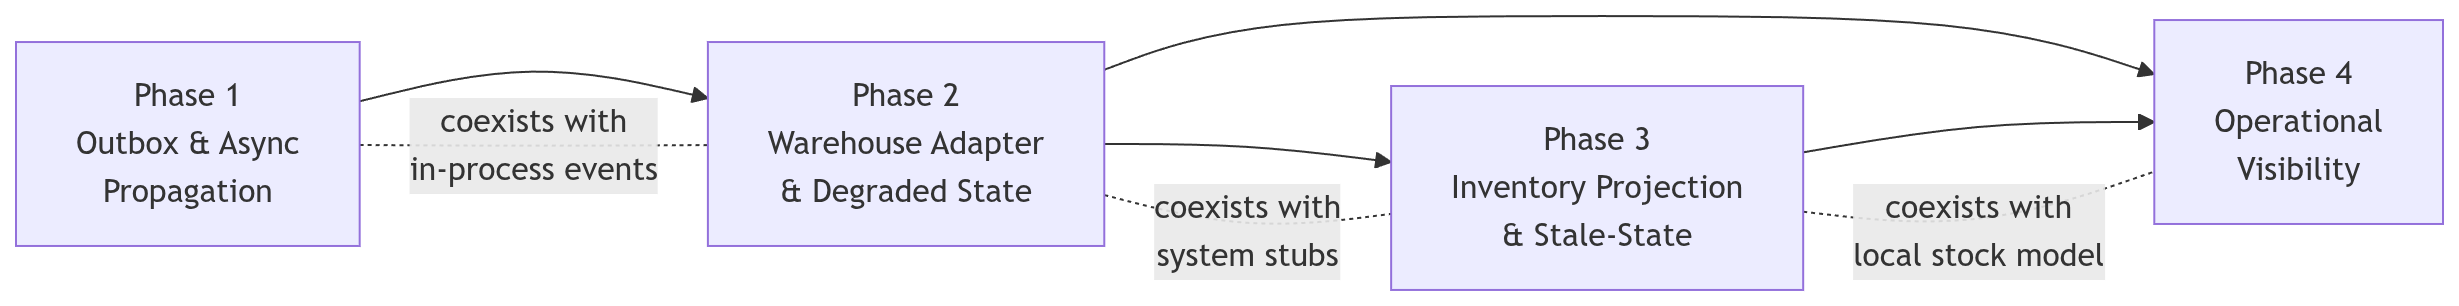
\includegraphics[width=\textwidth]{images/evolution-roadmap.png}
\caption{Implementation phases, ordering, and coexistence constraints.}
\label{fig:evolution-roadmap}
\end{figure}

\subsection{Phase 1: Outbox and Asynchronous Propagation}

An outbox table is added to the nopCommerce database. Order placement writes an integration
task in the same transaction as the order, and a scheduled task publishes unpublished records
to the integration layer. This phase has no dependency on any external system; the publication
destination can be a stub or log sink. What matters is proving the atomicity guarantee and the
publishing lifecycle before any adapter is built on top.

During this phase, the outbox coexists with the existing in-process event bus. The
\texttt{OrderPlacedEvent} continues to fire for internal reactions such as cache invalidation
and email notifications. The outbox adds a durable external path alongside it, not in place
of it.

\subsection{Phase 2: Warehouse Adapter and Degraded-State Handling}

With a working outbox, the Warehouse Adapter is built and connected. This phase introduces the
retry policy, idempotency key handling, and the integration state model: pending, sent,
accepted, delayed, failed, and recovered. A warehouse simulator stands in for the real system
and can be made slow or unavailable on demand, which is also how the mandatory pressure point
from the scenario is demonstrated.

The shipping adapter follows the same pattern and can be introduced in parallel with this
phase. System stubs coexist with the adapters throughout; real warehouse or carrier systems
are not required to validate the architecture.

\subsection{Phase 3: Inventory Projection and Stale-State Visibility}

The existing nopCommerce stock model is extended with source and freshness metadata. The
Inventory Adapter receives stock updates from warehouse and store systems and updates the
projection. When stock data is stale or conflicting, the model exposes a detectable state
rather than silently serving an outdated number. Detected conflicts are recorded for
reconciliation.

The local stock records that nopCommerce already manages are not replaced. The projection adds
a visibility layer on top of them. Checkout continues to revalidate stock using the existing
model; the projection is what operators and the storefront use to communicate freshness and
discrepancy state.

\subsection{Phase 4: Operational Visibility}

The operational read model aggregates the integration states produced in Phases 2 and 3 and
exposes them through the nopCommerce admin area or an equivalent support-facing view. This
phase introduces no new integration logic. Its purpose is to make earlier states visible and
actionable: which orders are awaiting warehouse confirmation, which fulfillment requests have
failed, and which inventory records are pending reconciliation.
